\chapter{METODOLOGI PENELITIAN}
\label{chap:metodologipenelitian}

% Ubah bagian-bagian berikut dengan isi dari desain dan implementasi

Untuk mencapai tujuan dalam tugas akhir ini, dilakukan beberapa tahap yang dimulai dengan memahami fenomena \textit{ground resonance} pada helikopter melalui studi pustaka serta teori pendukung. Berikutnya adalah melakukan perumusan terhadap permasalahan yang akan diselesaikan, dalam hal ini adalah terkait dengan fenomena \textit{ground resonance} helikopter modifikasi PTDI. Terdapat 3 pekerjaan yang dikerjaan secara paralel dan berurutan, yaitu pengukuran di tanah \textit{ground test} helikopter, perhitungan matematis secara teori dan komputasi Matlab serta simulasi menggunakan \textit{software} Femap. 

\begin{figure}[H]
	\centering
	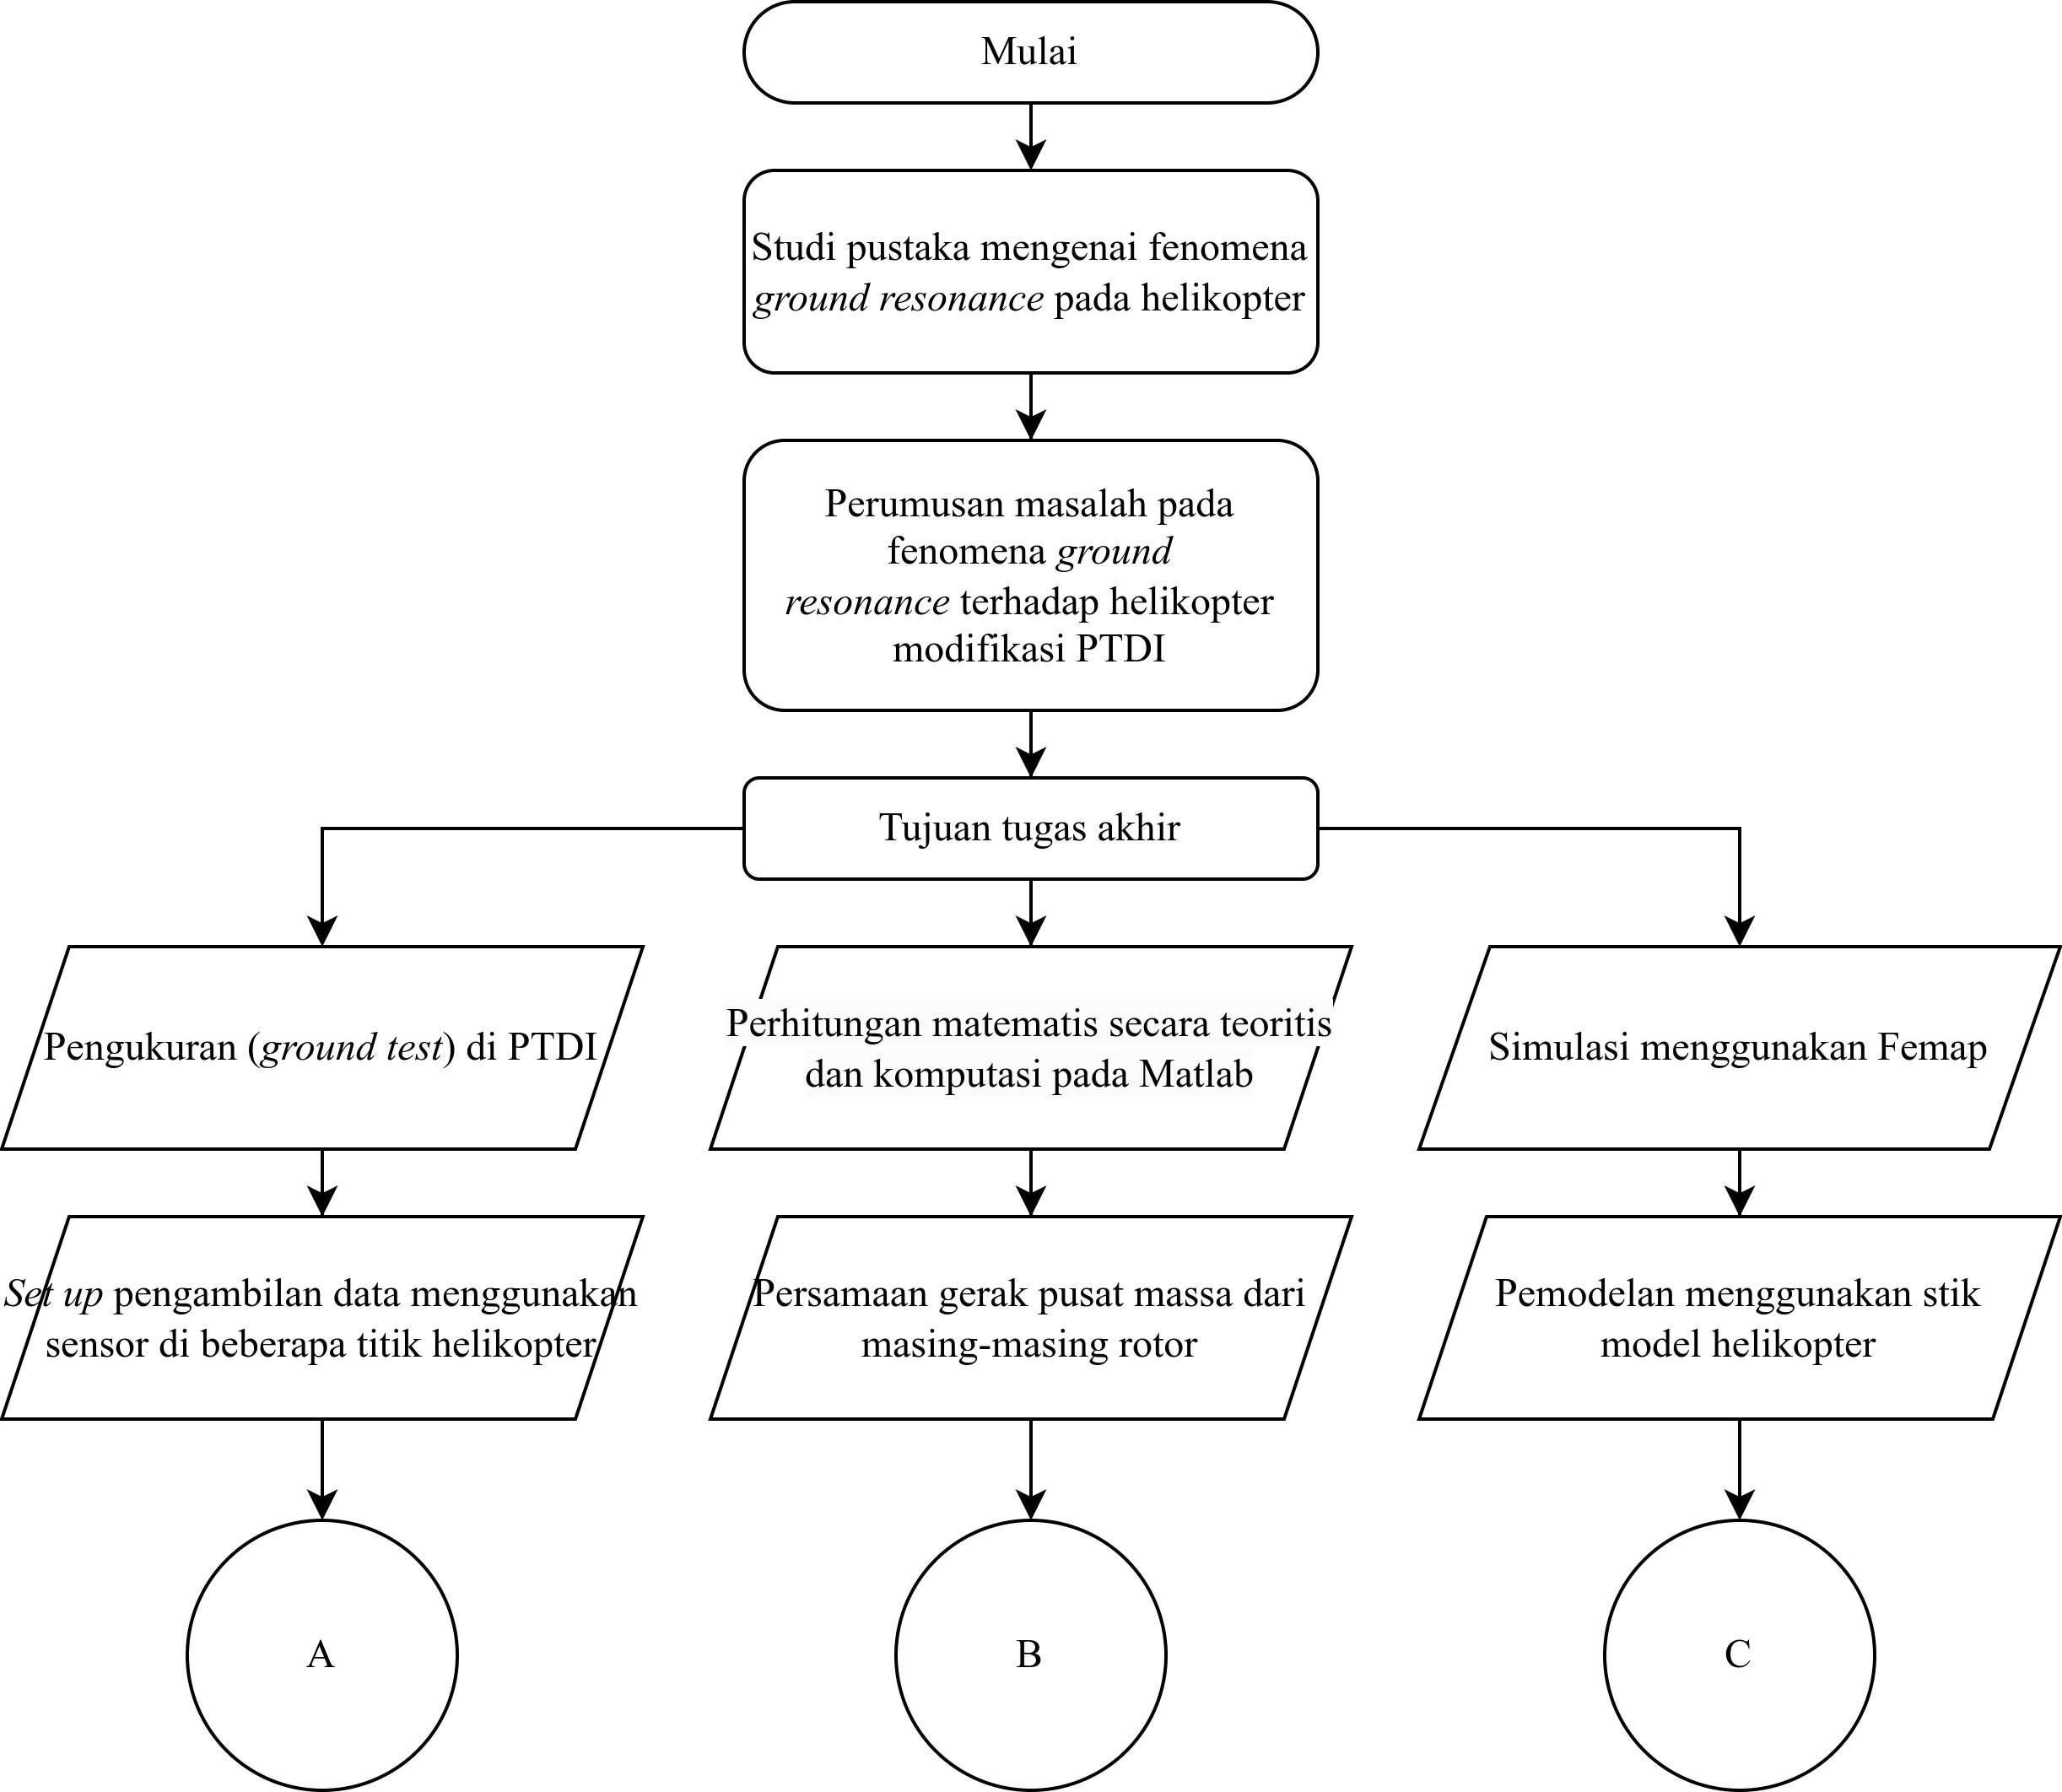
\includegraphics[width=1\linewidth]{gambar/TA_flow-Page-1.jpg}
	\caption{Diagram alir pengerjaan Tugas Akhir bagian 1.}
	\label{fig:TA_flow-Page-1.jpg}
\end{figure}

\begin{figure}[H]
	\centering
	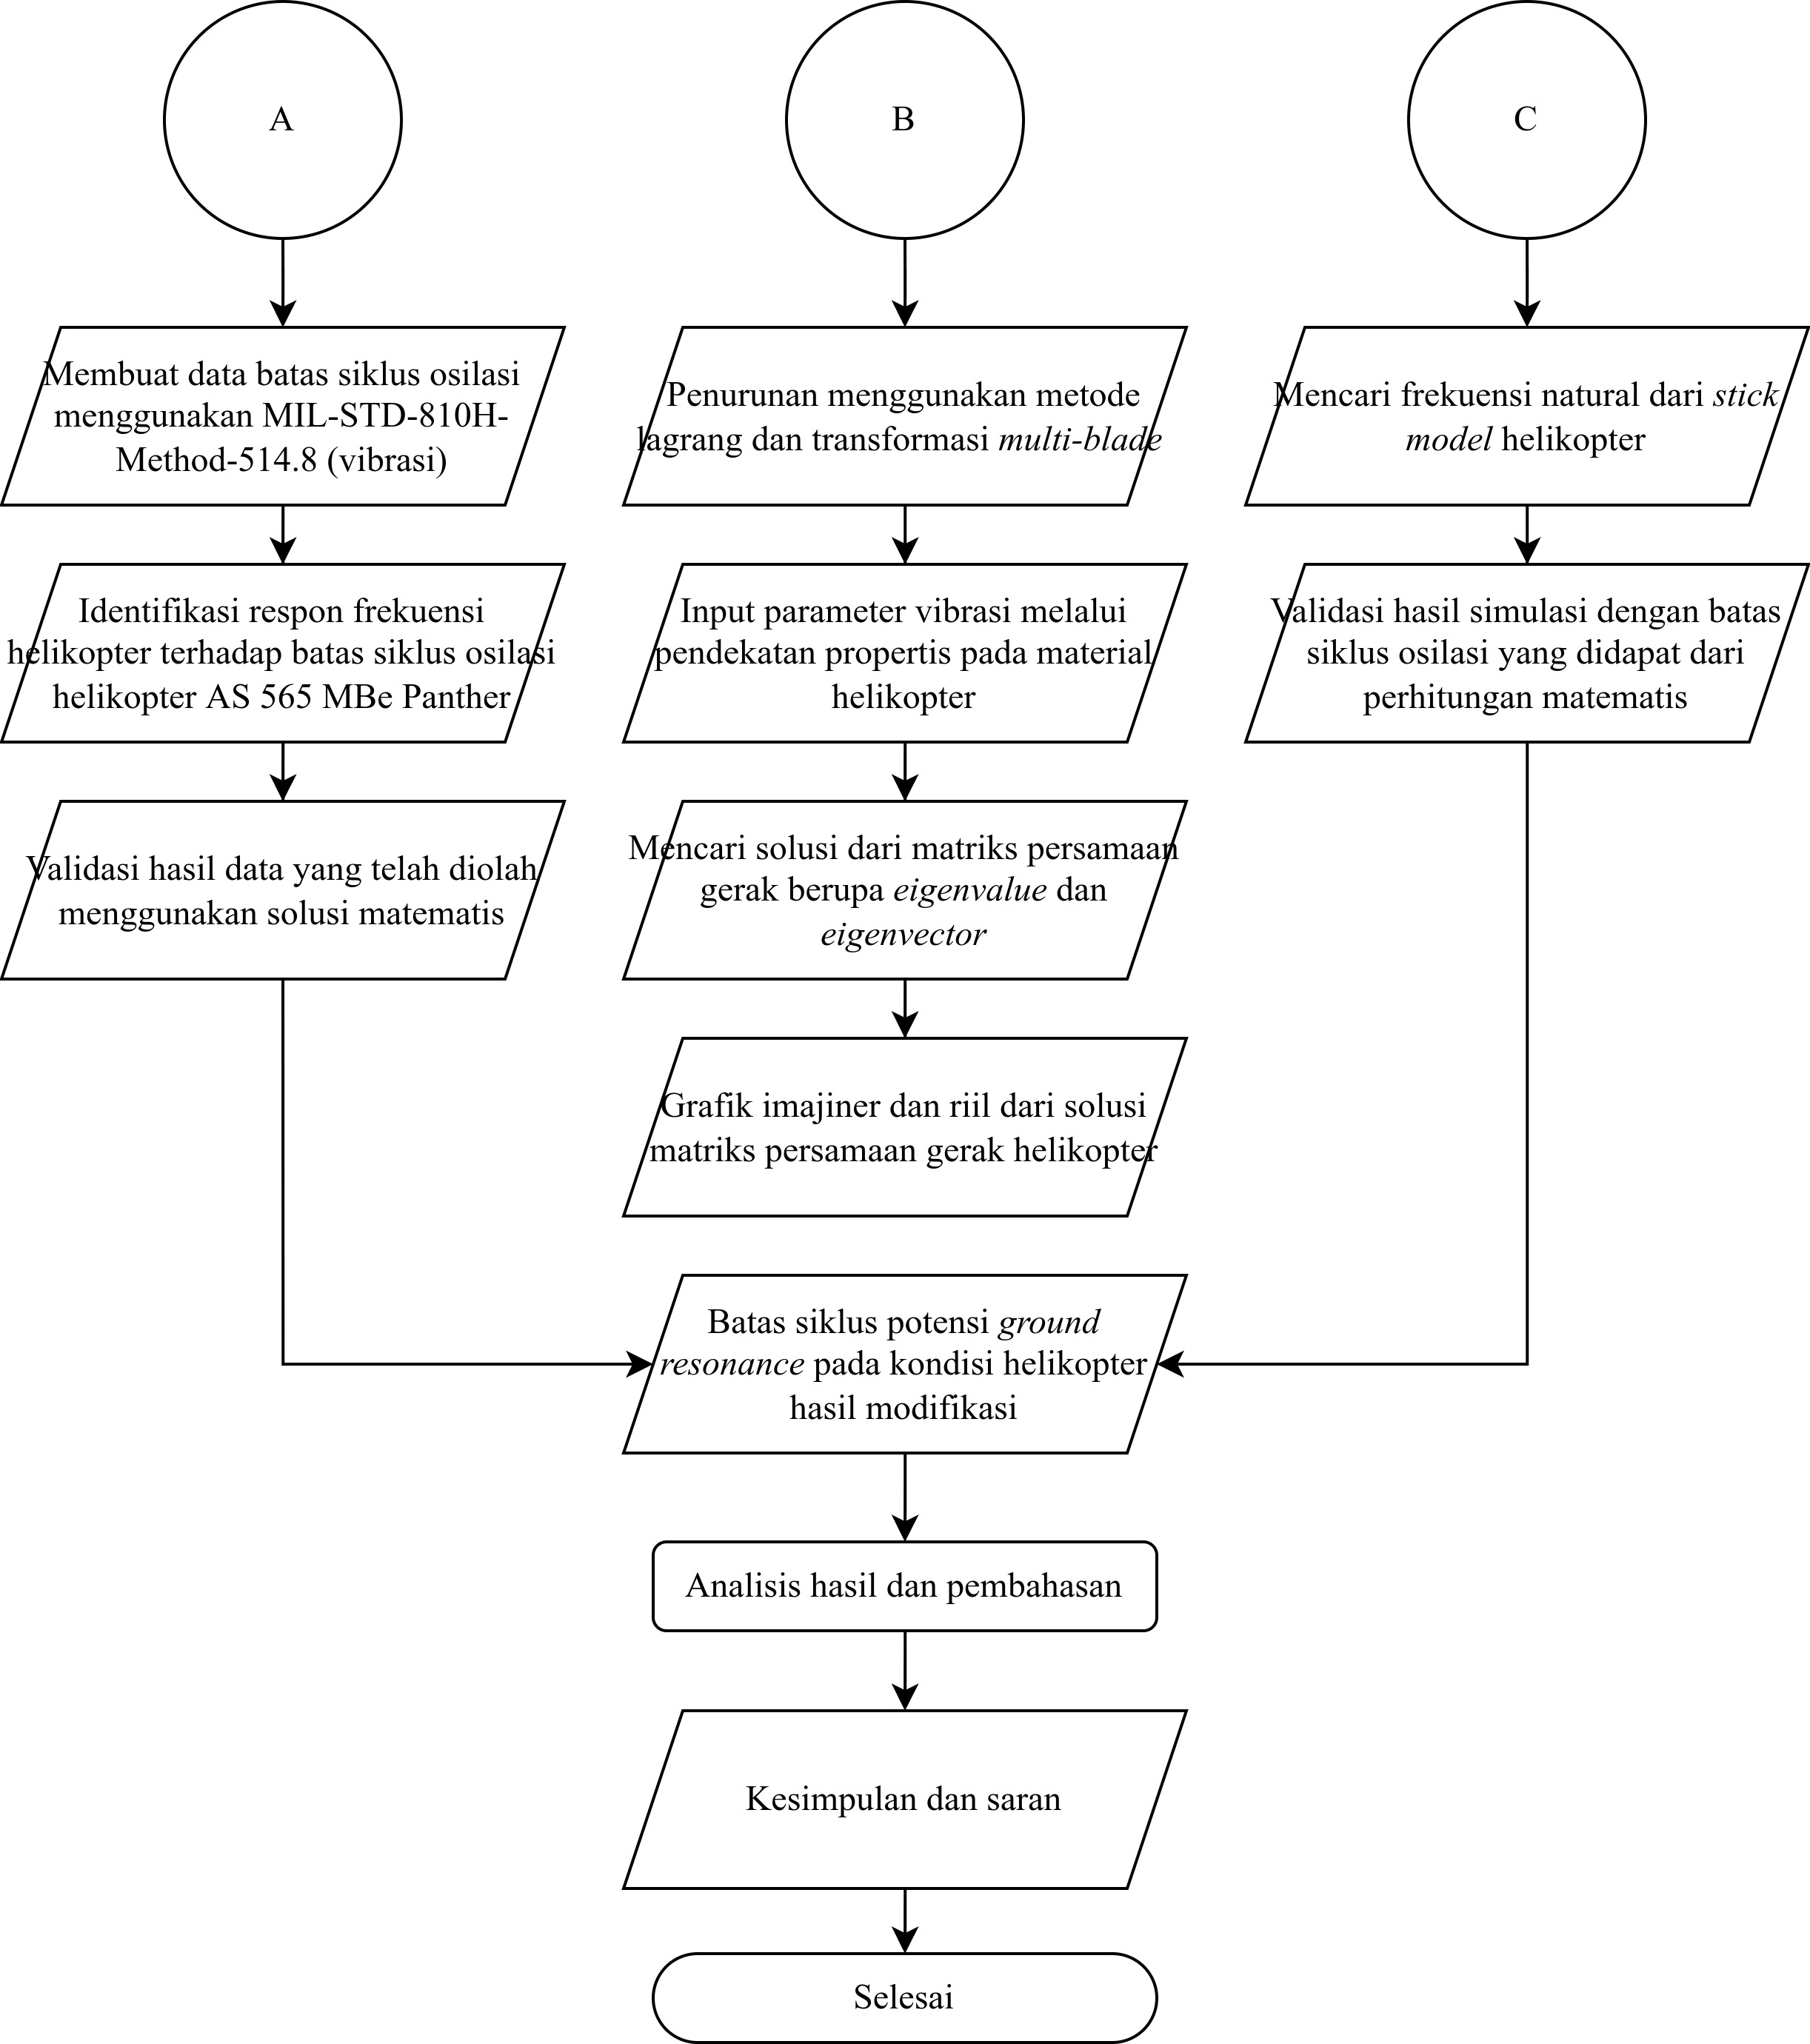
\includegraphics[width=0.95\linewidth]{gambar/TA_flow-Page-2.jpg}
	\caption{Diagram alir pengerjaan Tugas Akhir bagian 2.}
	\label{fig:TA_flow-Page-2.jpg}
\end{figure}

\section{Studi Pustaka}
\label{sec:studipustaka}

Studi pustaka merupakan tahap untuk membaca dan memahami referensi solusi serta metode peneliti sebelumnya berkaitan dengan \textit{ground resonance} pada helikopter. Beberapa referensi yang mendukung terhadap topik ini adalah mengenai metode pengolahan data hasil pengukuran menggunakan MIL-STD-810H-Method-514.8 (vibrasi), perhitungan matematis yang menggunakan konsep dasar dari parameter pegas-peredam-massa, penyelesaian matematis dengan menggunakan lagrang, transformasi \textit{multiblade} matriks, dan solusi eigen dengan bantuan komputasi Matlab. Kemudian referensi lain berupa informasi untuk pemakaian \textit{software} Femap dalam aspek simulasinya.

\section{Pengambilan Data \textit{Ground Test}}
  \label{sec:pengukurandata}

Pengambilan data \textit{ground test} dilakukan dengan mengikuti mekanisme yang telah ditetapkan oleh PTDI. Terdapat 2 pengukuran yang dilakukan, pertama adalah pengukuran terhadap \textit{damping ratio} dari respon helikopter terhadap impuls yang diberikan oleh pilot. Kedua, adalah pengukuran yang didapatkan menggunakan sensor akselerometer yang dipasangkan di beberapa titik pada helikopter.

\subsection{Pengukuran \textit{Damping Ratio}}
Pengukuran \textit{damping ratio} didapatkan dari \textit{Flight Test Instrumentation System} (FTIS). Respon terhadap impuls lateral serta longitudinal oleh pilot digunakan untuk mengetahui redaman getaran pada struktur helikopter. Nilai \textit{logarithmic decrement} didapatkan dari hasil pengukuran oleh FTIS dengan melihat seberapa cepat amplitudo getaran helikopter teredam sepanjang waktu setelah diberi impuls oleh pilot, nilai ini nantinya akan digunakan untuk menghitung \textit{damping ratio} helikopter.

\subsection{Pengukuran Data Vibrasi Akselerometer}
Pengukuran vibrasi dengan menggunakan akselerometer dilakukan dibeberapa titik pada helikopter. Konfigurasi mengenai peletakan sensor akselerometer dapat dilihat pada gambar dan tabel dibawah ini.

\begin{figure}[H]
	\centering
	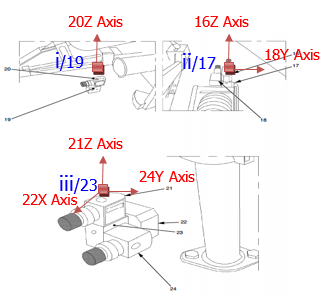
\includegraphics[width=0.53\linewidth]{gambar/peletakan_sensor.png}
	\caption{Peletakan akseleromter pada Helikopter.}
	\label{peletakan_sensor.png}
\end{figure}

\begin{longtable}{|c|c|}
	\caption{Lokasi dan arah akseleromter.}
	\label{tb:lokasiakselero}                        	\\
	\hline
	\textbf{Channel} & \textbf{Lokasi akselerometer} 	\\
	\hline
	1            	 & Kursi pilot (20Z)             	\\
	\hline
	2			     & Bagian luar stik kopilot (16Z)   \\
	\hline
	3				 & Bagian luar stik kopilot	(18Y)   \\
	\hline
	4				 & Frame 9" (21Z)                   \\
	\hline
	5				 & Frame 9" (22X)					\\
	\hline
	6				 & Frame 9" (24Y)					\\
	\hline
\end{longtable}

Kemudian berikut ini merupakan skema Helikopter AS 565 MBe Panther yang digunakan beserta keterangan dimensi dari beberapa arah skema.

\begin{figure}[H]
	\centering
	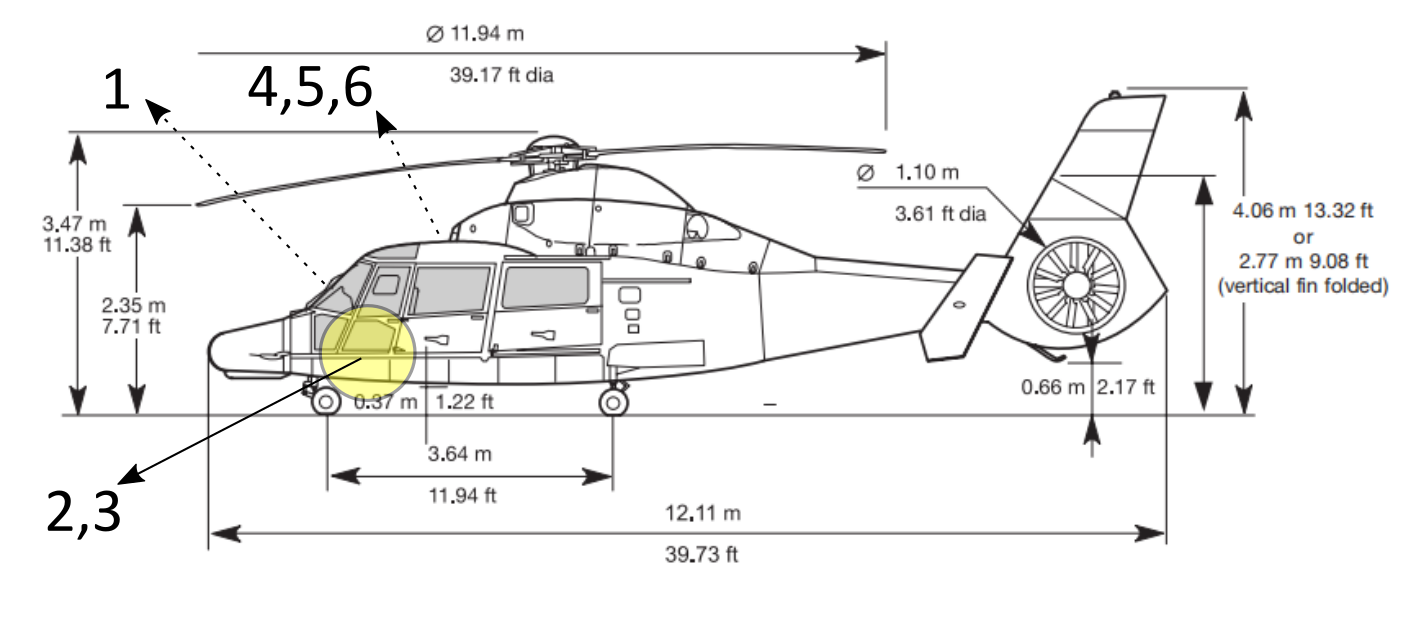
\includegraphics[width=0.8\linewidth]{gambar/tampak_samping.png}
	\caption{Skema dan dimensi helikopter AS 565 MBe Panther (tampak samping).}
	\label{tampak_samping.png}
\end{figure}

\begin{figure}[H]
	\centering
	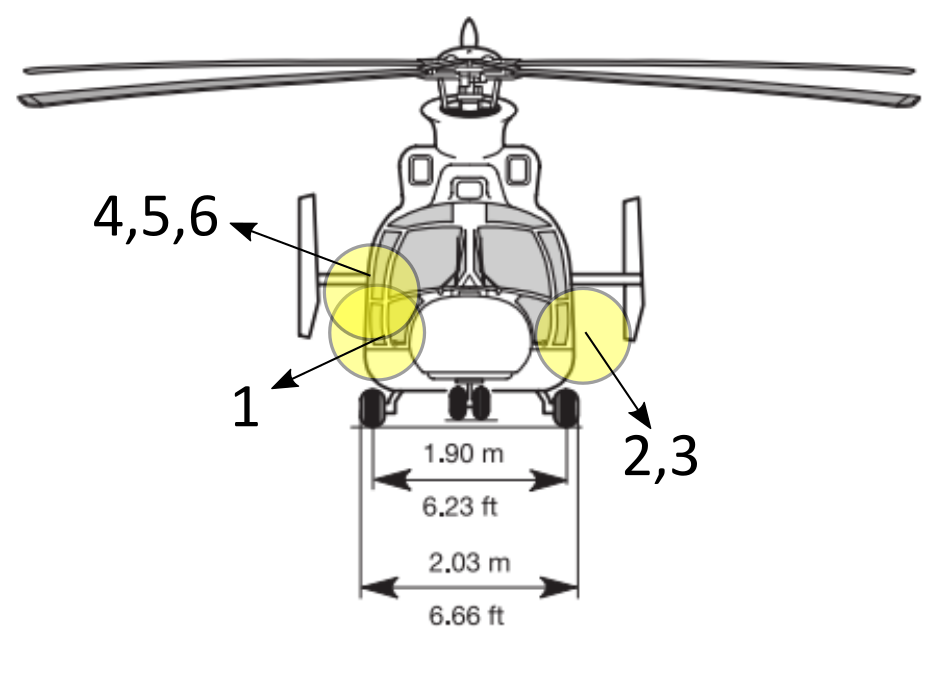
\includegraphics[width=0.6\linewidth]{gambar/tampak_depan.png}
	\caption{Skema dan dimensi helikopter AS 565 MBe Panther (tampak depan).}
	\label{tampak_depan.png}
\end{figure}

\begin{figure}[H]
	\centering
	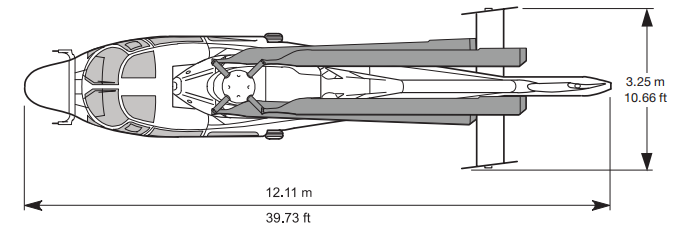
\includegraphics[width=0.8\linewidth]{gambar/tampak_atas.png}
	\caption{Skema dan dimensi helikopter AS 565 MBe Panther (tampak atas).}
	\label{tampak_atas.png}
\end{figure}

Tabel 3.2. merupakan variasi pada \textit{landing gear absorbers}. Variasi tersebut dilakukan pada bagian ban dan oleo helikopter. Propertis mengenai variasi \textit{landing gear absorbers} ditampilkan pada tabel 3.3. Selanjutnya pada tabel 3.4. memberikan informasi yang berkaitan dengan variasi \textit{input} pada \textit{ground test}. Secara teknis, dalam 1 kondisi pengujian terdapat 12 variasi \textit{input} yang diberikan kepada helikopter. 

\begin{longtable}{|c|c|c|c|c|c|} 
	\caption{Variasi \textit{Landing gear absorbers.}}
	\label{tb:variasilanding}								\\	
	\hline
	\multirow{3}{3em}{\centering \textbf{Kondisi ke-}}&\multicolumn{5}{|c|}{\textbf{Kondisi Pengujian}} \\
	\cline{2-6}
	& \textbf{NLG }& \multicolumn{2}{|c|}{\textbf{LH MLG}} & \multicolumn{2}{|c|}{\textbf{RH MLG}}\\
	\cline{2-6}
	& \textbf{Oleo/Tyre }&\textbf{Oleo}&\textbf{Tyre}&\textbf{Oleo }& \textbf{Tyre }\\
	\hline
	1 &	Nominal/Nominal & Nominal & Nominal & Nominal & Nominal \\
	\hline
	2 & Nominal/Nominal & High	  & High	& High	  & Nominal \\
	\hline
	3 & Nominal/Nominal & Nominal & Nominal	& High	  & High    \\
	\hline
	4 & Nominal/Nominal & Nominal & Nominal	& Low	  & Low	    \\
	\hline
	5 & Nominal/Nominal & Low	  & Low 	& Nominal & Nominal \\
	\hline
	6 & Nominal/Nominal & High	  & High	& High	  & High    \\
	\hline
	7 & Nominal/Nominal & Low	  & Low 	& Low	  & Low     \\
	\hline
	8 & Nominal/Nominal & High	  & High	& Low	  & Low     \\
	\hline
	9 & Nominal/Nominal & Low	  & Low	    & High	  & High 	\\
	\hline
	10 & Nominal/Nominal & High	  & High	& Nominal & High 	\\
	\hline
	11 & Nominal/Nominal & High	  & High	& Low	  & High 	\\
	\hline
\end{longtable}

\begin{longtable}{|c|c|c|m{0.3\linewidth}|}
	\caption{Propertis kuantitatif variasi \textit{landing gear absorbers} pada ban dan oleo helikopter.}
	\label{tb:propertiskuantitatif}								\\
	\hline
	\multirow{3}{*}{\centering NLG} & \multirow{2}{*}{\centering Oleo} & \multirow{2}{*}{Nominal} & Hydraulic: 10 bar (145 psi) \\
	\cline{4-4}
	&&& Nitrogen 30$^o$C=42 bar(psi)\\
	\cline{2-4}
	& Tyre & Nominal & 5.5 bar (79.7 psi)\\
	\hline
	\multirow{9}{*}{\centering MLG}&\multirow{6}{*}{\centering Oleo}& \centering \multirow{2}{*}{\centering Low}& Hydraulic: 10 bar (145 psi) \\
	\cline{4-4}
	&&& Nitrogen 15$^o$C: HP=49.0 bar (711 psi) LP=4.0 bar (59.0 psi) \\
	\cline{3-4}
	&& \centering Nominal & Hydraulic: 10 bar (145 psi) \\
	\cline{4-4}
	&&& Nitrogen 30$^o$C: HP=51.5 bar (747 psi) LP=4.2 bar (61 psi) \\
	\cline{3-4}
	&& \centering High & Hydraulic: 10 bar (145 psi) \\
	\cline{4-4}
	&&& Nitrogen 45$^o$C: HP=54.0 bar (783 psi) LP=4.4 bar (63.82 psi) \\
	\cline{2-4}
	& \centering Tyre & Low & 8.48 bar (123 psi)\\
	\cline{3-4}
	&& Nominal & 10.8 bar (156.6 psi)\\
	\cline{3-4}
	&& High & 13.1 bar (190 psi)\\
	\hline
\end{longtable}

\begin{longtable}{|c|c|c|c|c|}
	\caption{Variasi \textit{input} pada \textit{ground test} Helikopter.}
	\label{tb:variasi_input}									\\
	\hline
	\textbf{No.} & \textbf{SAS} & \textbf{Power} & \textbf{Input Control} & \textbf{Name of Sequence} \\
	\hline
	1 & \multirow{6}{*}{\centering OFF} & Ground Idle & Longitudinal & FILO \\
	\cline{1-1} \cline{3-5}
	2 && Ground Idle 			      & Lateral      & FILA \\
	\cline{1-1} \cline{3-5}
	3 && Flight Idle (on Ground)      & Longitudinal & FFLO \\
	\cline{1-1} \cline{3-5}
	4 && Flight Idle (on Ground)      & Lateral      & FFLA \\
	\cline{1-1} \cline{3-5}
	5 && Flight Idle (Light on Wheel) & Longitudinal & FLLO \\
	\cline{1-1} \cline{3-5}
	6 && Flight Idle (Light on Wheel) & Lateral      & FLLA \\
	\hline
	7 & \multirow{6}{*}{\centering ON}& Ground Idle  & Longitudinal & NILO \\
	\cline{1-1} \cline{3-5}
	8 && Ground Idle 				  & Lateral      & NILA \\
	\cline{1-1} \cline{3-5}
	9 && Flight Idle (on Ground)      & Longitudinal & NFLO \\
	\cline{1-1} \cline{3-5} 
	10 && Flight Idle (on Ground)     & Lateral      & NFLA \\
	\cline{1-1} \cline{3-5}
	11 && Flight Idle (Light on Wheel)& Longitudinal & NLLO \\
	\cline{1-1} \cline{3-5}
	12 && Flight Idle (Light on Wheel)& Lateral 	 & NLLA \\
	\hline
\end{longtable}

Semua data yang didapatkan pada hasil pengukuran \textit{damping ratio} dan vibrasi oleh akselerometer selanjutnya akan diolah dan dianalisis apakah helikopter AS 565 MBe Panther hasil modifikasi tersebut berpotensi mengalami fenomena \textit{ground resonance}. Sehingga helikopter dapat dikatakan aman untuk dapat digunakan sebagaimana kegunaannya setelah dimodifikasi. Kemudian, data vibrasi pada akselerometer akan dimasukkan pada batas siklus osilasi sesuai dengan acuan yang terdapat pada MIL-STD-810H-Method-514.8 (vibrasi).

\begin{figure}[H]
	\centering
	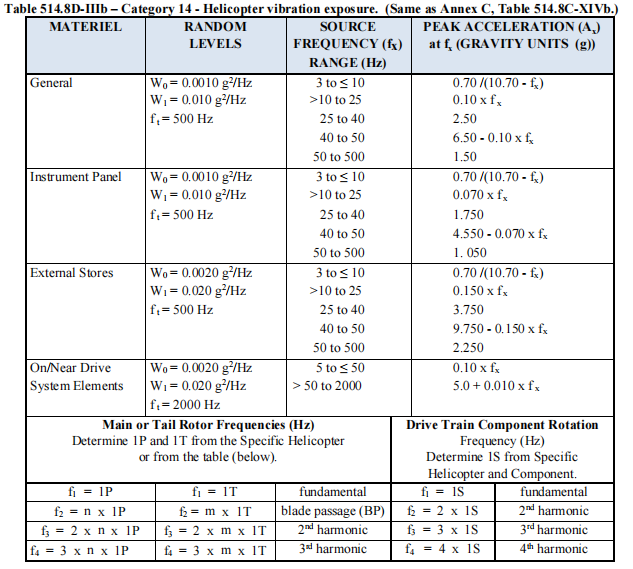
\includegraphics[width=0.8\linewidth]{gambar/MIL_STD.png}
	\caption{Gambar dari tabel acuan MIL-STD-810H-Method-514.8 untuk menghitung batas osilasi yang dimiliki oleh helikopter.}
	\label{fig:MIL_STD}
\end{figure}


\section{Pemodelan pada Femap}
	\label{sec:femap}
Dalam mencari solusi yang secara tepat merepresentasikan batas siklus osilasi pada perhitungan matematis. Berdasarkan referensi yang telah didapatkan, diperlukan langkah awal membuat skema pemodelan sederhana yang selanjutnya akan membantu untuk mendefinisikan posisi pusat massa dari masing-masing rotor pada helikopter. 